\chapter{Háttérismeretek}
\section{Modellek}
Terveket, modelleket az élet számos területén alkalmazunk, ugyanis ez által tudjuk még az előtt vizsgálni a megvalósítandó terméket, rendszert, hogy azt ténylegesen létre kellene hozni. A vizsgálat célja és módja egész sokféle lehet. A látvány tervező bemutat egy látványtervet és a megfelelő stakeholderek ezt értékelik, vagy egy rendszerről komplex matematikai módszerekkel kell eldönteni, hogy stabil-e. A modellek leírása sokféle módon történhet, de célszerű egy olyan jelölési rendszert alkalmazni, ami legalább az azonos téma területen belül, elfogadott és használt, hogy a többi szakember is értelmezni, vizsgálni tudja a modellt.

A jelölési rendszer vagy modellezési nyelv lehet egy szöveges leírás is, például egy programkód, de sokszor célszerű valamilyen vizuális megoldás használni azaz formák és nyilak illetve  szimbólumokat tartalmazó diagramokat alkalmazni. Ezek sok esetben kifejezőbbek, lényegre törőbbek, és elsősorban könnyebben értelmezhetőek mint a szöveges leírások.

\section{Statechart formalizmus}
Az állapottérkép egy állapotgép grafikus leírása, amit rendszerek állapot alapú viselkedésének leírásához használunk. Ez azt jelenti, hogy rendszert véges sok állapottal jellemezhetjük, amelyek közül adott időpillanatban néhány aktív. Az állapotok közötti átjárást állapotátmeneteknek hívjuk. Az állapotok és állapotátmenetek tulajdonképpen egy irányított gráfot definiálnak, ahol az állapotok csomópontok, az állapotátmenetek pedig irányított élek. A legtöbb esetben az állapotok közötti átjárás valamilyen feltételhez vagy feltételekhez kötöttek például egy esemény megérkezéséhez, vagy valamilyen logikai feltétel kielégüléséhez, ha a feltételek teljesülnek akkor tüzelésről beszélünk, ilyenkor az él vagy állapotátmenet kiindulási állapota inaktívvá, míg a célállapota aktívvá válik.

\subsection{MagicDraw állapottérképek}
Az előzőekben inkább általánosságban beszéltem az állapottérképekről, most az elemeinek a szintaktikáját és szemantikáját fogom ismertetni, méghozzá a UML 2 szerint amit a MagicDraw követ.

\begin{itemize}
	%--------------
	% Állapot
	%--------------
	\item \emph{állapot (state)}: az állapottérképek csomópontjai, a rendszer működésének egyfajta jól megkülönböztethető állásai, amelyek valamilyen esemény bekövetkezésére várnak. Az állapotok rendelkeznek:
	\begin{itemize}
		\item név: az állapot neve
		\item be/kilépési akció: be és kilépés során végrehajtandó cselekvés
	\end{itemize}
	
	%--------------
	% Állapot átmenet
	%--------------
	\item \emph{állapot átmenet (transition)}: az állapottérképek élei, az állapotok közötti átjárhatóságot definiálják, ha egy állapot átmenet érvényre jutását tüzelésnek hívjuk. Az állapotátmenetek rendelkeznek:
		\begin{itemize}
			\item triggerekkel
			\item őrfeltételekkel
		\end{itemize}
	%---------------
	% Trigger
	%---------------
	\item \emph{trigger}: állapot átmenet tüzelésének megkísérlése valamilyen esemény hatására, az esemény lehet
	\begin{itemize}
		\item Változás esemény (Change Event): valamilyen értéknek a megváltozása.
		\item Üzenet esemény (Message Event): valamilyen üzenet típusú objektumnak az érkezése, amit ebben a kontextusban kérésnek tekintünk. Egy ilyen típusú kommunikáció valójában kétféle eseménytől függ, az üzenet elküldésétől és annak küldőjétől és az üzenet fogadásától és annak fogadójától. A kérés lehet egy metódus hívás, egy jelnek (signal) a fogadása.
		\item Időzítés esemény (TimeEvent): idő változásához kötött esemény
	\end{itemize}
	Fontos megjegyezni, hogy itt most nem foglalkozok az események kiváltásának kérdésével azaz a küldő oldallal, és a fogadásnál sem térek ki a portokra, és interfészekre, ezek értelmezése és hasznossága az állapottérképek közti kommunikáció modellezése nélkül ezen a ponton elenyésző.
	%----------------
	% Guard
	%----------------
	\item \emph{őrfeltétel (guard)}: egy logikai kifejezés, melynek teljesülnie kell, hogy az állapotátmenet, amihez hozzá van rendelve tüzelhessen.
	%-----------------
	% Ábra: állapot-atmenet-trigger-guard-action
	%----------------
	\begin{figure}[!ht]
		\centering
		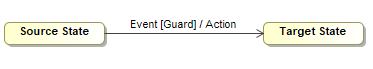
\includegraphics[keepaspectratio]{figures/statechart_elements/states.png}
		\caption{Állapotok és köztük definiált állapotátmenet, triggerrel, őrfeltétellel és actionnel}
	\end{figure}
	%----------------
	% Összetett állapot
	%----------------
	\item \emph{összetett állapot(composite state)}: összetett állapotról akkor beszélünk, ha az állapotnak vannak további belső állapotai is, ilyenkor, ha az állapotgép egy tüzelés hatására kilép a kompozit állapotból akkor a belső állapotokból is kilép.
	%------------------
	% Régió
	%------------------
	\item \emph{régió}: régió egy állapotokat tartalmazó egység, az állapottérkép mindig tartalmaz egy régiót amibe az állapotok definiálhatók. Régiók létezhetnek egymással párhuzamosan ilyenkor a végrehajtásuk párhuzamosan történik.
	%------------------
	% Ortogonális állapot
	%------------------
	\item \emph{ortogonális állapot (orthogonal state)}: olyan összetett állapot ami két vagy több régiót tartalmaz.
	%-------------------
	% Submachine state
	%-----------------
	\item \emph{submachine state}: egy olyan állapot, ami egy állapottérképre hivatkozik, ez lehetővé teszi, hogy egy állapottérkép többszöri felhasználását, akár más-más kontextusban, működését tekintve hasonló mint az ortogonális állapot
	%-----------------
	% Ábra
	%-----------------
	\begin{figure}[!ht]
		\centering
		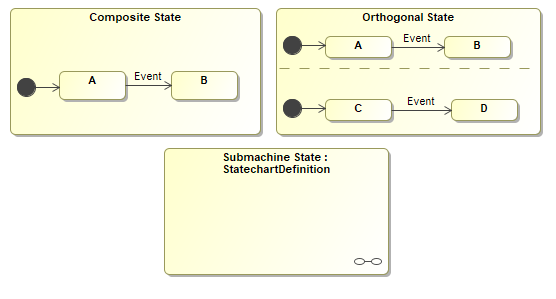
\includegraphics[keepaspectratio]{figures/statechart_elements/composit.png}
		\caption{Összetett állapot (balra), ortogonális állapot (jobbra) és submachine state (alul)}
	\end{figure}
	%-----------------
	% Kezdő állapot
	%-----------------
	\item \emph{kezdő állapot (initial state)}: A kezdő állapot egy pszeudo állapot, régiónként egy szerepelhet belőle és a régió belépési pontjaként szolgál.
	%-----------------
	% Végső állapot
	%-----------------
	\item \emph{végső állapot}\footnote{UML 2 ben a végső állapotot nem pszeduo állapotként hanem állapotként van definiálva https://www.omg.org/spec/UML/2.0} (final state): A végső állapot, a régió terminálasi pontja, ha egy állapotgép összes régiója egy végső állapotba ért akkor az állapotgép is terminál.
	%----------------
	% Termináló állapot
	%----------------
	\item \emph{termináló állapot (terminal state)}: pszeudo állapot, ami az egész állapotgépet azonnal terminálja
	%---------------
	% Belépési pont
	%---------------
	\item \emph{belépési pont(entry point)}: egy pszeudo állapot, ami egy állapotgép vagy egy kompozit állapot belépési pontját reprezentálja, célja egységbe zárni az állapotot vagy az állapotgépet. Továbbá léteznie kell egy állapotátmenetnek közte és egy az állapot vagy állapotgép régiója között.
	%--------------
	% Kilépési pont
	%---------------
	\item \emph{kilépési pont(exit point)}: mint a belépési pont, de ez kilépési pontot reprezentál
	%---------------
	% kapcsolódási pont
	%---------------
	\item \emph{kapcsolódási pont referencia(connection point reference)}: submachine stateben definiált be és kilépési pontokra tudunk vele hivatkozni, ez lehetővé teszi, hogy a submachine stateben leírt belső állapotokhoz is felvehessünk állapotátmeneteket
	%---------------
	% History state
	%--------------
	\item \emph{history state}: olyan pszeudo állapot, amely egy régióban megjegyzi az utolsó aktív állapotot, a régióbol történő kilépéskor, ha a régióba visszalépünk a history state visszaállítja a megjegyzett állapotot. Amennyiben nincs előző állapot az ő belőle húzott állapotátmenet cél állapota lesz aktív. Létezik shallow és deep history state. Előbbi csak adott régión belül jegyzi meg az állapotot míg utóbbi a tartalmazott régiók állapotait is megjegyzi és visszaállítja.
	%-------------
	% Csomópont
	%-------------
	\item \emph{csomópont (junciton)}: több állapotátmenet összekapcsolása és egyként kezelése, például ha a cél állapotuk ugyan az és logikailag összetartoznak vagy egy beérkező átmenet szétbontása több átmenetre. Ilyenkor lehetőség van őrfeltételt rakni az átmenetekre, ezeknek a kiértékelése viszont még azelőtt történik, hogy bármelyik átmenet végrehajtásra kerülne, ezért egy ilyen ágat szokás statikus feltételes ágnak nevezni.
	%------------
	% Elágazás
	%-----------
	\item \emph{választás (choice)}: hasonló mint a csomópont, viszont az őrfeltételek az elágazásba való belépéskor értékelődnek ki dinamikusan. Ezt jellemzően alternatív útvonalak megadására használjuk. Fontos megjegyezni, hogy az elágazás és a csomópont esetében is lehetséges, hogy több átmenet is tüzelhetne, ilyenkor az érvényre jutó átmenet kiválasztása nem determinisztikus módon történik ezért elkerülendő, például else őrfeltétel alkalmazásával.
	%---------
	% Fork
	%---------
	\item \emph{fork}: pszeudo állapot, ami egy beérkező átmenetet szétbont több átmenetre, amiknek a cél állapotuk ortogonális régiókban találhatók. A kimenő átmeneteken nem lehet se trigger, sem pedig őrfeltétel.
	%---------
	% Join
	%---------
	\item \emph{join}: pszeudo állapot, ami több beérkező átmenetet kapcsol össze eggyé. Az átmenetek orthogonális régiókból kell, hogy induljanak és nem lehet rajtuk trigger vagy őrfeltétel. A join szinkronizációs funkcionalitással bír: addig nem lehet tovább lépni belőle amíg minden belé érkező átmenet végre nem hajtódott.
	%------------
	% Ábra: fork - join
	%-----------
	\begin{figure}[!ht]
		\centering
		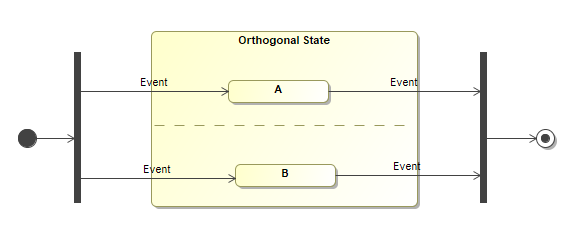
\includegraphics[keepaspectratio]{figures/statechart_elements/forkjoin.png}
		\caption{Példa: fork-join}
	\end{figure}
	
\end{itemize}

\section{MagicDraw}
A MagicDraw a No Magic nevű cég által fejlesztett modellező eszköz, amivel a modellek előállításán kívül lehetőségünk van ezeket szimulálni, validálni, vagy akár kóddá alakítani. Az eszköz első sorban UML modelleket lehet készíteni, de pluginnal lehetőségünk van SysML modelleket is készíteni. A SysML egy általános-célú modellezési nyelv ami az UML egy részhalmazának a kiterjesztésével keletkezett. A SysML 9 diagramtípus támogat, amelyből néhány UML ben is létezik. Ezek:
\begin{itemize}
	\item \emph{Block Definíciós Diagram (BDD)}
	\item \emph{Internal Block Diagram (IBD)}
	\item Package Diagram
	\item Use Case Diagram
	\item Activity Diagram
	\item Sequence Diagram
	\item \emph{State Machine Diagram (Statechart)}
	\item Parametric Diagram
\end{itemize}
Az állapottérképeket vagy \emph{statechartokat} én mint SysML modellek részeként vizsgálom, tehát a \emph{statechart} egy ún. \emph{Block} viselkedéseként van megadva.